% =====================================================================
%  FCCM 2027 submission draft -- double-blind.
%  Build: pdflatex admm_fccm; bibtex admm_fccm; pdflatex x2
% =====================================================================
\documentclass[conference]{IEEEtran}
\usepackage{amsmath,amssymb,amsthm}
\usepackage{booktabs}
\usepackage{graphicx}
\usepackage{tikz}
\usetikzlibrary{arrows.meta,positioning,fit}
\usepackage[hidelinks]{hyperref}
\usepackage{cite}

\newtheorem{theorem}{Theorem}
\newtheorem{proposition}{Proposition}

\begin{document}

\title{Degenerate-Set Annihilation: Predicting\\Fixed-Point Error in FPGA ADMM Solvers}

\author{\IEEEauthorblockN{Anonymous Authors}
\IEEEauthorblockA{Submission for double-blind review}}

\maketitle

\begin{abstract}
Fixed-point wordlength selection for FPGA optimization solvers rests on the
classical model in which every quantization contributes independent noise of
power $q^2/12$. We show that this model is wrong for proximal operators in a
specific, measurable way: on the operator's \emph{degenerate set}, where its
derivative vanishes, injected quantization error is annihilated exactly, so
effective error scales with $(1-d)$ for degenerate fraction $d$. The resulting
model matches bit-exact measurement to 0.99 (soft-threshold) and 1.00 (box
projection) on average over $d\in[0.12,0.88]$, where the classical error grows
as $1/(1-d)$: 3--4$\times$ averaged over that range, 900$\times$ at $d=0.999$. It transfers unchanged to a second
problem, LASSO, at 0.98--1.03 with $d$ up to 0.77. It explains the datapath width that a bit-exact sweep selects for an ADMM
accelerator on Artix-7, which we measure on routed silicon: narrowing Q2.16 to
Q2.9 removes 44.9\% of LUTs, raises $F_{\max}$ by 28.8\%, and cuts dynamic
energy per solve from 184 to 117\,nJ, from activity-annotated power, with
detection BER statistically unchanged. Both designs run bit-exact on a board at their in-context $F_{\max}$,
where the speed-up is 26.9\%. Narrowing a single operator's lane, by contrast, costs 3.7--4.1\% area at two
widths and buys no resolvable power or frequency. We state where the model
stops: it predicts ensemble behaviour, not per-instance worst cases.
\end{abstract}

% =====================================================================
\section{Introduction}

An FPGA accelerator for a proximal splitting method such as ADMM~\cite{boyd2011admm}
must fix a number format for every signal. Too few fraction bits and the solver
returns a wrong answer; too many and area, critical path and switching energy
all grow. Designers therefore either simulate exhaustively or reason with the
classical model, in which each rounding is an independent additive source of
power $q^2/12$~\cite{widrow2008quant} propagated through the algorithm.

That model is known to be inaccurate in feedback loops and under
correlated quantizations~\cite{lopez2007interval,naud2012correlation}, and the incumbents of
recent search-based wordlength optimization note that analytical noise
models remain limited to linear time-invariant systems~\cite{ha2020scalable,ha2023accuracy}. A proximal operator
is neither linear nor smooth. Jerez et al., analysing fixed-point ADMM on FPGA,
observe that the projection step can only \emph{reduce} error, by a diagonal
factor with entries in $[0,1]$ --- and then set that factor to the identity to
keep their bound conservative~\cite{jerez2014mpc}. Kinsman and Nicolici note that
their bit-width constraints assume no correlation between error and value, and
that a known correlation ``can be captured into
constraints''~\cite{kinsman2011iterative}.

This paper quantifies the factor that was discarded and supplies the
correlation that was missing. Our contributions:
\begin{enumerate}
\item \textbf{An operator error model} in which the degenerate set of a
proximal operator annihilates a measurable fraction $(1-d)$ of injected
quantization error (Theorem~\ref{thm:t1}), validated to 0.99/1.00 against
bit-exact simulation, with a stated 12\% miss on the coefficient term of the
one operator without a degenerate set.
\item \textbf{Transfer to a second problem.} The same model holds on LASSO's
native distribution (0.98--1.03, $d$ up to 0.77, off-lattice threshold), and
the accelerator runs LASSO bit-exact, on a board, with no change.
\item \textbf{A measured design point.} Selected by bit-exact sweep and
explained by the model, a Q2.9 datapath on Artix-7 saves 44.9\% of LUTs and
36\% of dynamic energy per solve against Q2.16, with unchanged detection BER, at 28.8\% higher $F_{\max}$ out of context and
26.9\% higher in context, bit-exact on a board at speed.
\item \textbf{A negative result.} Narrowing one operator's lane below the
main width --- the asymmetry an operator-level model invites --- costs area at
both widths tested and buys no resolvable power or frequency.
\end{enumerate}
We do not claim the first error model for fixed-point ADMM (Jerez et al.\ have
one), a worst-case bound, or that the width follows analytically without
simulation. Section~\ref{sec:limits} states where the model stops.

% =====================================================================
\section{Background and related work}
\label{sec:related}

\paragraph{ADMM with proximal lanes} For
$\min_x \tfrac12\lVert Hx-y\rVert^2+g(x)$ in scaled form,
\begin{align}
x^{k+1} &= M\,(q+\rho(z^k-u^k)), \nonumber\\
z^{k+1} &= \operatorname{prox}_{g/\rho}(x^{k+1}+u^k), \label{eq:admm}\\
u^{k+1} &= u^k+x^{k+1}-z^{k+1}. \nonumber
\end{align}
with $M=(H^{\top}H+\rho I)^{-1}$ and $q=H^{\top}y$. The x-update is a dense
mat-vec with a matrix fixed per problem; the z-update is elementwise. We study three proximal operators~\cite{parikh2014prox}:
soft-threshold $S_\kappa(v)=\operatorname{sgn}(v)\max(|v|-\kappa,0)$ (L1),
projection onto $[\ell,h]$ (Box), and ridge scaling $\gamma v$ (L2).

\paragraph{Error analysis of fixed-point ADMM} Jerez et al.\ derive a converging
upper bound on accumulated round-off for fixed-point ADMM on FPGA and use it to
choose a uniform fraction width~\cite{jerez2014mpc}; their bound discards the
projection's attenuating factor, which is the quantity we measure. The
Heriot-Watt line bounds inexact proximal methods under errors assumed additive,
bounded and, in~\cite{hamadouche2022sharper}, zero-mean and orthogonal to the
iterate~\cite{hamadouche2022inexact,hamadouche2022sharper}. Degenerate-set
annihilation violates that orthogonality by construction: which coordinates are
annihilated depends on the iterate. Our model is a refinement of theirs, and it
is predictive where theirs are bounds.

\paragraph{Wordlength optimization} Analytical methods for LTI
systems~\cite{constantinides2003wordlength} and search methods for general
ones~\cite{ha2020scalable,ha2023accuracy} are mature; for iterative
computations, Kinsman and Nicolici allocate widths by SMT with conjugate
gradient as the case study, and their robust widths reach single to double
precision after input-space restriction~\cite{kinsman2011iterative}. Li et
al.\ set the methodological bar we adopt --- an analytical model validated
against bit-exact simulation to under 1\,dB, with measured hardware ---
for a different, linear algorithm~\cite{li2023fam}.

\paragraph{Mixed precision} Wu et al.\ report up to 67\% LUT and 60\% power
reduction for mixed-precision ADMM~\cite{wu2022mixed}. Those figures are
against an FP32 baseline, with power from the vendor estimator, and vary
precision over iterations; ours vary it over operators, against a fixed-point
baseline, with activity-annotated power. In their fixed-point ADMM rows the
mixed configuration saves DSPs (21 vs.\ 30) but uses slightly more LUTs (6807
vs.\ 6775): non-uniform precision is not free in fabric there either.

% =====================================================================
\section{The error model}
\label{sec:model}

\subsection{Degenerate-set annihilation}

Let $P_\theta$ be a proximal operator with parameter $\theta$, applied
elementwise and evaluated in a lane with $W$ fraction bits, $q=2^{-W}$. Split
the input coordinates into the degenerate set $D=\{i:\partial P/\partial v_i=0\}$
and its complement, and write $d=|D|/n$ and $L$ for the slope on $D^c$.

\begin{theorem}[Operator error decomposition]\label{thm:t1}
Let the lane round its input to the lattice, $\tilde v=v+e$ with $e$ uniform on
$[-q/2,q/2)$ and independent of $v$; let $P$ be piecewise affine in $v$ with
finitely many breakpoints, slope $0$ on $D$ and $L$ on $D^c$; let $v$ have a
bounded density near the breakpoints, with $d=\Pr(v\in D)$; and let $\theta$ be
held as $\tilde\theta=\theta+\delta_\theta$ with $\delta_\theta=O(q)$. Then the per-coordinate output error
$e_P=P_{\tilde\theta}(\tilde v)-P_\theta(v)$ satisfies
\begin{equation}
\mathbb{E}\,e_P^2=(1-d)\Big[L^2\frac{q^2}{12}+\sigma^2_{\theta,D^c}\Big]
+d\,\sigma^2_{\theta,D}+O(q^3),
\label{eq:t1}
\end{equation}
where $\sigma^2_{\theta,S}=\mathbb{E}[(\partial P/\partial\theta)^2\,|\,v\in S]\,\delta_\theta^2$.
If the output is not on the lattice (a product, as in L2), add its rounding,
$q^2/12$.
\end{theorem}

\begin{proof}
Condition on $v$. If $v$ lies in the interior of $D^c$ at distance more than
$q/2+|\delta_\theta|$ from every breakpoint (so that neither the input nor the
parameter rounding moves $v$ across one), $\tilde v$ stays on the same affine piece and
$e_P=Le+(\partial P/\partial\theta)\delta_\theta$; since $\mathbb{E}e=0$ the
cross term vanishes and $\mathbb{E}[e_P^2\,|\,v]=L^2q^2/12+(\partial P/\partial
\theta)^2\delta_\theta^2$. If $v$ lies in the interior of $D$, equally far from
every breakpoint, $P$ is constant in $v$ on the whole interval reachable by $e$, so
the input error is removed exactly and only
$(\partial P/\partial\theta)\delta_\theta$ remains. The remaining inputs lie
within $q/2$ of a breakpoint, a set of probability $O(q)$ by the density bound,
on which $|e_P|\le Lq/2+|\partial P/\partial\theta||\delta_\theta|$; with
$\delta_\theta=O(q)$ they contribute $O(q^3)$. Averaging over $v$ gives
\eqref{eq:t1}.
\end{proof}

The theorem is operator-level: one application of $P$ to an input carrying
fresh rounding error, which is how a lane sees it each iteration; error
accumulated around the loop is the subject of Sect.~\ref{sec:loop}. Equivalently,
$(1-d)L^2=\mathbb{E}[P'(v)^2]$ is the operator's first-order perturbation gain.
What matters for a proximal operator is that this expectation is set by $d$,
which the data, the parameter and the iterate determine, and which in our
workloads ranges from 0 to above 0.9. Concretely, with $\delta_\theta$ the
rounding error of $\theta$ on the lane lattice: for L1, $L=1$, $\sigma^2_{\theta,D^c}=\delta_\kappa^2$ and
$\sigma^2_{\theta,D}=0$; for Box, $L=1$, $\sigma^2_{\theta,D^c}=0$ and
$\sigma^2_{\theta,D}$ is the squared rounding error of whichever bound clips;
for L2, $d=0$, $L=\gamma$, and the coefficient error enters as
$\mathbb{E}[v^2]\,\delta_\gamma^2$. The classical model charges every
coordinate $L^2q^2/12$, so with an on-lattice parameter it overestimates by
$1/(1-d)$. That is not a constant
correction: $d$ is set by the data, the parameter and the iterate.

\subsection{Validation against bit-exact simulation}

We measure each operator in isolation, on inputs harvested from floating-point
ADMM runs, against a bit-exact model of the RTL (Fig.~\ref{fig:t1}). Sweeping
each operator's parameter moves $d$ across $[0,1]$; parameters are placed on
the lattice so that the $\theta$ terms vanish and annihilation is isolated.
Over $d\in[0.17,0.88]$ for L1 and $[0.12,0.83]$ for Box, prediction/measured
is 0.991 and 1.004 on average (0.979--1.020 per point), while the
classical model is off by 3.8$\times$ and 3.0$\times$ on average --- 1.1--1.2$\times$
at the low end of the range, 903$\times$ at $d=0.999$, and infinitely at $d=1$,
where the measured error is exactly zero. Very close to $d=1$ the residual
error is a handful of boundary events and the ratio becomes noisy (0.96 at
$d=0.999$, 0.69 at $d=0.9999$). On the solver's own operating distribution,
averaged over $W=6$--12, the model gives 0.99 (L1) and 1.00 (Box). For L2 it gives 0.88:
with $d=0$ the annihilation term is inactive and the 12\% miss lies in the
coefficient term, which this result does not validate to better than 12\%.
In bits, the model errs by 0.007 (L1), 0.000 (Box) and 0.092 (L2), inside the
0.17-bit (1\,dB) bar of~\cite{li2023fam}. Table~\ref{tab:t1} collects the
validation.

\begin{table}[t]
\centering\footnotesize\setlength{\tabcolsep}{3pt}
\caption{Theorem~\ref{thm:t1} vs.\ bit-exact measurement}
\label{tab:t1}
\begin{tabular}{llccc}
\toprule
operator & input distribution & $d$ & T1/meas & classical/meas \\
\midrule
L1  & sweep, on-lattice & 0.17--0.88 & 0.991 & 3.8$\times$ \\
Box & sweep, on-lattice & 0.12--0.83 & 1.004 & 3.0$\times$ \\
Box & sweep, on-lattice & 0.999     & 0.96  & 903$\times$ \\
L1  & detection solver          & 0.00      & 0.99  & 0.61$^a$ \\
Box & detection solver          & 0.18      & 1.00  & 0.95 \\
L2  & detection solver          & 0         & 0.88  & 0.21$^a$ \\
L1  & LASSO solver, 5 $\lambda$ & 0.62--0.77 & 0.98--1.03 & 1.6--2.7$\times$ \\
\bottomrule
\end{tabular}\\[2pt]
\raggedright\scriptsize $^a$Below 1: with $d\approx0$ there is nothing to
annihilate, and parameter rounding ($\kappa$, $\gamma$) adds error the
classical model omits.
\end{table}

\begin{figure}[t]
\centering
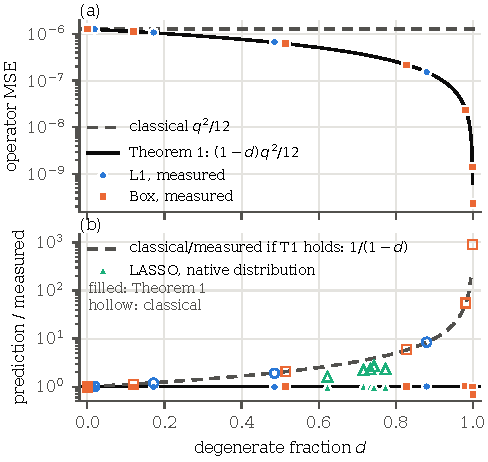
\includegraphics[width=\columnwidth]{fig_t1.pdf}
\caption{Theorem~\ref{thm:t1} against bit-exact measurement. (a) L1 and Box
error as each operator's parameter moves $d$ across $[0,1]$ ($W=8$,
on-lattice): measurement follows $(1-d)q^2/12$, not the classical flat
$q^2/12$; at $d=1$ it is exactly zero (not plotted on the log axis).
(b) The same as ratios, with LASSO on its native distribution
(Sect.~\ref{sec:lasso}), where the off-lattice threshold adds a parameter term
that the model includes and the classical model does not.}
\label{fig:t1}
\end{figure}

\subsection{Two consequences for design}

\paragraph{Lattice rule} If $\theta$ is not on the lane's lattice, its rounding
error $\delta$ enters every coordinate where the output depends on $\theta$,
and for $|\delta|\sim q/2$ it dominates~\eqref{eq:t1}. Placing operator
constants on the lattice is worth one bit: measured 3.68--3.90$\times$ error
against a predicted 4$\times$, and one bit through the closed loop.

\paragraph{Range feasibility} The datapath must represent
$M=(H^{\top}H+\rho I)^{-1}$, whose entries satisfy $|M_{ij}|\le1/\rho$, a bound
approached as $H^{\top}H$ becomes singular.
\begin{proposition}\label{prop:rho}
Representing $M$ in Q$I$.$F$ for every $H$ requires $\rho>2^{-(I-1)}$; with
$I=2$, $\rho>0.5$ (or $\rho=0.5$ with one-LSB saturation of $M$).
\end{proposition}
We registered this before measuring it. On the detection workload, $\max|M|$ is
2.91 at $\rho=0.125$ (unrepresentable in Q2.$F$) and 1.34 at $\rho=0.5$; on an
underdetermined generator, where $H^{\top}H$ is singular, it reaches 1.99 at
$\rho=0.5$, against the bound of 2. We use $\rho=1$.

\subsection{From operator to solver}
\label{sec:loop}

Operator error is amplified by the ADMM loop by a gain $G$. For the
contractive L2 lane, $\log G=a\log R+c$ with $R=\lVert(I-T)^{-1}\rVert$ the
resolvent of the linearized iteration predicts solver-level error to 0.046\,bits
on problem instances \emph{disjoint} from those it was fitted on. The gain
itself is the point, more than its variation: $G$ moves only between 6.4 and
12.1 across 300$\times$ of conditioning, because contraction pins the resolvent,
so a single constant already does well (0.094\,bits); ignoring the loop
($G=1$) under-predicts by 1.65\,bits. Adding one bit to the prediction covers
99\% of random held-out instances ($+0.66$ at the 99th percentile), but not an
adversarial search, which finds $+1.12$.
For L1 and Box, fitted loop-gain forms that looked accurate under
cross-validation on the fitting instances (0.34 and 0.23\,bits) fail on
disjoint instances (1.38 and 0.73\,bits); we retract them and claim only the
operator-level model for these lanes. Table~\ref{tab:heldout} shows why
cross-validation on the same instances could not see it. For L1, a single
instance carries 68\% of the ensemble error in the median cell, and the
ensemble mean varies by 0.59\,bits (s.d.) between instance sets --- more than
the fit's own error. For Box, the held-out error is 4.7$\times$ its
instance-set variability: the fit is over-fitted, not noisy. A criterion cannot be
tighter than the quantity's repeatability; we therefore hold loop-level claims
to 0.5\,bits on held-out instances, the resolution of an integer width
decision.

\begin{table}[t]
\centering\footnotesize\setlength{\tabcolsep}{4pt}
\caption{Loop-gain model: fitted vs.\ disjoint instances (bits)}
\label{tab:heldout}
\begin{tabular}{lcccc}
\toprule
lane & in-sample & held-out & instance-set s.d. & p99 per instance \\
\midrule
L1  & 0.279 & 1.382 & 0.593 & $+1.90$ \\
Box & 0.146 & 0.734 & 0.156 & $+3.46$ \\
L2  & 0.061 & \textbf{0.046} & 0.075 & $+0.66$ \\
\bottomrule
\end{tabular}
\end{table}

% =====================================================================
\section{From model to datapath}
\label{sec:width}

The model's job is to say where to look and why; a bit-exact sweep confirms the
choice. We sweep the main fraction width $F$ with all lanes tied to it, on
8-variable problems ($32\times8$ real BPSK detection, $\rho=1$), and record the
smallest $F$ whose solution NMSE against double precision meets a target, with
saturation counters required to stay at zero (otherwise the sweep measures
clipping, not quantization).

Table~\ref{tab:width} gives the result. At NMSE $10^{-4}$ every operator
needs $F=9$; at $10^{-3}$, $F=8/7/7$ for L1/Box/L2; at $10^{-5}$, $11/10/10$.

\begin{table}[t]
\centering\footnotesize
\caption{Minimum main width $F$ meeting an NMSE target (no saturation)}
\label{tab:width}
\begin{tabular}{lccc}
\toprule
NMSE target & L1 & Box & L2 \\
\midrule
$10^{-3}$ & 8 & 7 & 7 \\
$10^{-4}$ & \textbf{9} & \textbf{9} & \textbf{9} \\
$10^{-5}$ & 11 & 10 & 10 \\
\midrule
$10^{-4}$, lanes pinned 8/7/8 & 9 & 9 & 9 \\
\bottomrule
\end{tabular}
\end{table} We take Q2.9 (11 bits) as the design
point. The operators differ by at most one bit at any target. At
$10^{-4}$, lanes pinned at 8/7/8 need exactly the same $F$ as lanes tied to it,
so narrowing individual lanes costs no accuracy there; at $10^{-5}$ the pinned
lanes cannot reach the target at any $F$, and lane width binds. Whether
narrowing buys area is what Section~\ref{sec:asym} tests in fabric. We make no
claim here about which operator needs the most precision.

\paragraph{Application quality} NMSE against double precision is a proxy;
detection accuracy is what the application sees. Table~\ref{tab:ber} gives
uncoded BER for the Box (detection) lane over 24\,000 bits per SNR, through
the same bit-exact datapath that was measured on silicon. We registered two
predictions. Double-precision BER lies within the 95\% confidence interval of
the Q2.9 estimate at every SNR: it does. Q2.9 makes the same decision as double precision on at
least 99.9\% of bits: it does at every SNR except 0\,dB, where it agrees on
99.896\% (25 bits of 24\,000) --- a miss as registered, at a BER of 3\%.

\begin{table}[t]
\centering\footnotesize\setlength{\tabcolsep}{4pt}
\caption{Uncoded BER, BPSK $32\times8$, 24\,000 bits per SNR}
\label{tab:ber}
\begin{tabular}{rcccc}
\toprule
SNR (dB) & ridge$^a$ & ADMM, double & Q2.16 & Q2.9 \\
\midrule
0  & $4.06\cdot10^{-2}$ & $3.16\cdot10^{-2}$ & $3.16\cdot10^{-2}$ & $3.22\cdot10^{-2}$ \\
2  & $2.00\cdot10^{-2}$ & $1.26\cdot10^{-2}$ & $1.26\cdot10^{-2}$ & $1.28\cdot10^{-2}$ \\
4  & $8.42\cdot10^{-3}$ & $2.42\cdot10^{-3}$ & $2.42\cdot10^{-3}$ & $2.42\cdot10^{-3}$ \\
6  & $4.17\cdot10^{-3}$ & $3.33\cdot10^{-4}$ & $3.33\cdot10^{-4}$ & $3.75\cdot10^{-4}$ \\
8  & $1.37\cdot10^{-3}$ & $4.17\cdot10^{-5}$ & $4.17\cdot10^{-5}$ & $4.17\cdot10^{-5}$ \\
10--14 & $\ge7.1\cdot10^{-4}$ & 0 & 0 & 0 \\
\bottomrule
\end{tabular}\\[2pt]
\raggedright\scriptsize $^a$Signs of the x-update alone, $(H^{\top}H+I)^{-1}H^{\top}y$:
a linear detector with fixed regularization, whose high-SNR floor is residual
inter-symbol interference, not noise.
\end{table}

In use, the model explains the sweep's result and says where to look; it
does not replace the sweep.
Proposition~\ref{prop:rho} fixes $\rho$ against the integer width; the
lattice rule fixes the operator constants; Theorem~\ref{thm:t1}, with $d$
measured from a floating-point run, gives each lane's operator-level error at
a candidate $W$, and so which lane can be narrowed at what cost; for the
contractive lane the loop model plus its one-bit margin gives the solver-level
width. A bit-exact sweep over representative instances then confirms the
choice, as Table~\ref{tab:width} does here.

% =====================================================================
\section{Architecture}
\label{sec:arch}

\begin{figure}[t]
\centering
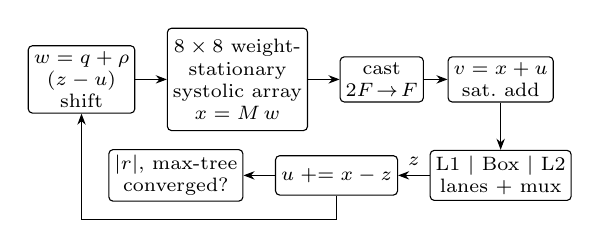
\begin{tikzpicture}[font=\scriptsize, >={Stealth[length=4pt]},
  blk/.style={draw, rounded corners=1.5pt, minimum height=5mm, inner sep=2pt, align=center},
  every node/.style={align=center}]
\node[blk, minimum width=17mm, minimum height=13mm] (arr) {$8\times8$ weight-\\stationary\\systolic array\\$x=M\,w$};
\node[blk, left=4mm of arr] (pre) {$w=q+\rho$\\$(z-u)$\\shift};
\node[blk, right=4mm of arr] (cast) {cast\\$2F\!\to\!F$};
\node[blk, right=3mm of cast] (v) {$v=x+u$\\sat.\ add};
\node[blk, below=6mm of v, minimum width=16mm] (prox) {L1 $\mid$ Box $\mid$ L2\\lanes + mux};
\node[blk, left=4mm of prox] (dual) {$u\mathrel{+}=x-z$};
\node[blk, left=4mm of dual] (res) {$\lvert r\rvert$, max-tree\\converged?};
\draw[->] (pre) -- (arr);
\draw[->] (arr) -- (cast);
\draw[->] (cast) -- (v);
\draw[->] (v) -- (prox);
\draw[->] (prox) -- node[above]{$z$} (dual);
\draw[->] (dual) -- (res);
\draw[->] (dual.south) |- ++(0,-3mm) -| (pre.south);
\end{tikzpicture}
\caption{Datapath. All signals Q2.$F$; products accumulate at $2F$ and are cast
back. $\rho$ is a power of two, so the pre-combination is a shift. Each
iteration is 26 cycles; a solve of $K$ iterations is $26K+3$.}
\label{fig:arch}
\end{figure}

The accelerator (Fig.~\ref{fig:arch}) maps~\eqref{eq:admm} directly. $M$ is
loaded once per problem into an $8\times8$ weight-stationary systolic array
whose input vector is pipelined down the columns and whose partial sums
accumulate along the rows; ADMM is sequentially dependent, so there is one
vector in flight and no input skew. With $\rho$ a power of two the
pre-combination is a shift. The three proximal lanes are all instantiated and
selected at run time, so that a lane cannot be removed by constant
propagation and inflate a reported saving. Convergence is tested on
$\lVert r\rVert_\infty$ through a balanced max-tree; with the threshold scaled
by $1/\sqrt N$ this is sufficient for the $\ell_2$ criterion, and avoids $N$
multipliers and a square root.
Every arithmetic primitive saturates rather than wraps, and a bit-exact Python
model mirrors each one.

Each iteration takes 26 cycles, the array's $2N+2=18$ plus the vector
stages, and a solve of $K$ iterations takes exactly $26K+3$ cycles in every
build we measured. Cycles per iteration are independent of every width
parameter, so all of the speed difference between builds comes from
$F_{\max}$. Our validation runs set the convergence threshold to zero, so the
early exit fires when the residual quantizes to exactly zero --- stagnation,
which comes sooner at coarser precision (15/19/12 iterations at Q2.9 against
28/32/22 at Q2.16). Those counts describe termination, not convergence, and we
quote every throughput and energy figure at a fixed $K=32$.

% =====================================================================
\section{Hardware results}
\label{sec:hw}

\subsection{Method}

Artix-7 XC7A35T, Vivado 2025.2, out-of-context implementation of the core. Area
is Slice LUTs from \texttt{report\_utilization}, the metric comparators
report. $F_{\max}$ is found by binary search on the clock constraint with a
full implementation at each step, reported as $1/T$ for the tightest period
$T$ that met timing --- never as $1/(T-\text{slack})$. Power is post-route,
annotated with switching activity from a gate-level simulation of the
regression vectors (SAIF), at Vivado's \emph{High} confidence with 72--75\% of
nets matched; every such simulation also checks the output bit-exact against
the golden model. The vectorless estimate for the same builds was about
10$\times$ too high. Reports round to 1\,mW, which bounds every power ratio we
quote. Every figure in this section is regenerated by committed scripts, and a
fresh run reproduces all seven builds exactly.

\subsection{The design point}

\begin{table}[t]
\centering\footnotesize
\caption{Q2.16 vs.\ the Q2.9 design point (Artix-7, routed)}
\label{tab:headline}
\begin{tabular}{lrrr}
\toprule
 & Q2.16 & Q2.9 & change \\
\midrule
Slice LUTs                      & 4673 & 2574 & $-44.9\%$ \\
\quad proximal lanes            & 2159 & 1032 & $-52.2\%$ \\
Flip-flops                      & 2199 & 1359 & $-38.2\%$ \\
DSP48 / BRAM                    & 64 / 0 & 64 / 0 & --- \\
$F_{\max}$, out of context      & 66.3\,MHz & 85.4\,MHz & $+28.8\%$ \\
$F_{\max}$, in context (board)  & 65\,MHz & 82.5\,MHz & $+26.9\%$ \\
Dynamic power (SAIF)            & 11\,mW & 7\,mW & --- \\
Dynamic energy / solve, $K=32$ & 184\,nJ & 117\,nJ & $-36\%$ \\
\bottomrule
\end{tabular}
\end{table}

Table~\ref{tab:headline} gives the result. Narrowing the datapath from Q2.16 to
Q2.9 removes 44.9\% of LUTs, more than half of them in the proximal lanes.
$F_{\max}$ rises 28.8\%; the binary search resolution bounds the ratio at
$+27.6\%$ to $+30.4\%$. Dynamic power falls from 11 to 7\,mW; with 1\,mW
rounding the reduction lies between 29 and 44\%. Dynamic energy per solve
combines the measured power, the measured cycle count and the measurement
clock (50\,MHz): $P_{\text{dyn}}\cdot(26K+3)/f$ gives 184 and 117\,nJ at
$K=32$. It inherits the same rounding --- the $-36\%$ is bounded at 29--44\%
--- but not a dependence on clock: energy per cycle is frequency-independent,
so the figure holds at whatever clock a reader assumes. Device static power is 68\,mW
in both builds, so \emph{total} on-chip power falls only from 80 to 76\,mW; we
claim the dynamic reduction only.

The speed-up has a structural cause. Across all seven builds the critical
path falls into two families with no overlap: through a proximal lane
(21--24 logic levels, 63.9--68.9\,MHz) or through the convergence test
(16--17 levels, 79.7--86.5\,MHz). At Q2.16 the lane binds; at Q2.9 the lanes
are short enough that the convergence test binds instead. Narrowing a lane
below the main width inserts a cast on the lane path, and two bits of it are
enough to return the lane to the slow family: at the same 10-bit main width,
8-bit lanes reach 68.9\,MHz against 79.7 for 10-bit lanes. (A 1-bit cast at
$F=9$ is not.)

\begin{table}[t]
\centering\footnotesize\setlength{\tabcolsep}{2.8pt}
\caption{All seven builds (routed; power from SAIF, 50\,MHz).
Path: critical path through a proximal lane (A) or the convergence test (B).}
\label{tab:builds}
\begin{tabular}{lcccccc}
\toprule
$F$ & lanes & LUT & lanes' LUT & FF & $F_{\max}$ & dyn mW / path \\
\midrule
16 & 16/16/16 & 4673 & 2159 & 2199 & 66.3 & 11 / A \\
16 & 8/8/8    & 3259 & 1020 & 1975 & 67.6 & 10 / A \\
16 & 8/7/8    & 3392 & 1153 & 1975 & 63.9 & 10 / A \\
10 & 10/10/10 & 3043 & 1272 & 1479 & 79.7 &  7 / B \\
10 & 8/8/8    & 2698 &  976 & 1447 & 68.9 &  7 / A \\
\textbf{9} & \textbf{9/9/9} & \textbf{2574} & \textbf{1032} & \textbf{1359} & \textbf{85.4} & \textbf{7 / B} \\
9  & 9/8/9    & 2669 & 1128 & 1359 & 86.5 &  7 / B \\
\bottomrule
\end{tabular}
\end{table}

\begin{figure}[t]
\centering
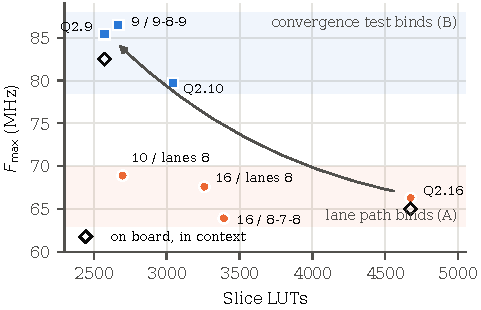
\includegraphics[width=\columnwidth]{fig_builds.pdf}
\caption{$F_{\max}$ against area for the seven builds. Critical paths fall into
two families with no overlap; the Q2.16$\to$Q2.9 step crosses between them.
Diamonds: the two headline builds on the board, timing met in context.}
\label{fig:builds}
\end{figure}

Table~\ref{tab:builds} and Fig.~\ref{fig:builds} show all seven builds. The four whose
critical path is the lane path stay in 63.9--68.9\,MHz however their lanes are
set; $F_{\max}$ rises only when the lane path stops binding.

\subsection{On the board, at speed}

Out-of-context figures exclude the clock network and I/O. To test whether the
headline survives a complete design, we wrapped both builds for a Basys3 board
--- problems from ROM, results over UART --- clocked each from one MMCM at an
exact frequency, and swept downward. A bitstream was written only for the
highest frequency meeting setup and hold after routing, in context. Q2.16 met
65\,MHz and missed 66.25; Q2.9 met 82.5\,MHz and missed 85. At those clocks
both builds return results bit-exact against the golden vectors for all three
operators. The speed-up in context is 26.9\% at the met points, bracketed
$+24.5\%$ to $+30.8\%$ by the step size, overlapping the out-of-context bracket:
the frequency gain belongs to the datapath, not to the measurement method.
(A first bring-up used a fabric clock divider behind a LUT multiplexer; it
produced correct results at 50\,MHz but fails in-context timing by 5.7\,ns,
because both clocks reach the clock net. We report only the MMCM builds.)

\subsection{Lane area is linear in width}
\label{sec:cost}

Fitting $A_{\text{lane}}(W)=bW+c$ on the three builds whose lanes equal the
main width ($W=16,10,9$) gives $b=19.6$ LUT/bit per proximal instance and
predicts the held-out $W=8$ build at the same cast depth to $-6.3\%$. A quadratic fit, exact on the same three points,
predicts it to $-21.6\%$ with a negative quadratic coefficient, so we reject it:
at lane granularity, casts, comparators and saturating adders dominate, and
only the L2 lane contains a multiplier. A second $W=8$ build, with deeper
casts into a 16-bit main path, is predicted to $-10.4\%$. Narrowing all lanes
together pays: 8-bit lanes at $F=16$ use 1020 LUTs against 2159 for 16-bit
lanes.

\subsection{A negative result: per-operator asymmetry}
\label{sec:asym}

If lane area were quadratic in width, as multiplier-dominated datapaths
are~\cite{constantinides2003wordlength}, narrowing the lanes whose operators
tolerate it would pay. It is linear, so narrowing one lane by a bit saves a
fraction of $b$, while the narrowed lane needs a cast in and out of the main
width. We built matched pairs at two main
widths, identical except for one narrowed lane (L1/Box/L2 at 8/7/8 vs.\ 8/8/8
with $F=16$; 9/8/9 vs.\ 9/9/9 with $F=9$). Asymmetry \emph{increases} area by
4.1\% and 3.7\%, and the proximal lanes themselves by 13.0\% and 9.3\% (17 and
12 LUTs per proximal instance): the casts cost more than the bit saves.
Dynamic power is identical within each pair (10 vs.\ 10\,mW; 7 vs.\ 7\,mW), so
any difference is below the 1\,mW resolution, and $F_{\max}$ moves by
$-5.5\%$ and $+1.3\%$ --- inconsistent in sign, the latter one search step ---
so we claim no frequency effect. The result is scoped to what we built:
one lane narrowed by one bit, at two main widths. There it is a fabric loss
at both.

\subsection{A second problem: LASSO}
\label{sec:lasso}

LASSO, $\min\tfrac12\lVert Ax-b\rVert^2+\lambda\lVert x\rVert_1$, maps onto the
unchanged datapath with the L1 lane at $\kappa=\lambda/\rho$. We registered four
predictions before running it, for 2-sparse problems with Gaussian $A$ of $m$
rows. (i) The operator model holds on LASSO's native distribution: it gives
0.981--1.028 over five values of $\lambda$, at $d=0.62$--$0.77$ with the
threshold wherever $\lambda$ puts it, where the classical model is off by
1.6--2.7$\times$ (Fig.~\ref{fig:t1}b). This matters beyond scope: on the
detection workload the L1 lane sits at $d\approx0$, so this is the first test
of the $(1-d)$ factor for L1 at the solver's own threshold, on data it
produces itself. (ii) Width
need grows as rows are removed and $\lVert M\rVert_2\to1/\rho$ (Table~\ref{tab:lasso}):
$F^\star=8$ at $m=32$, 9 at $m=16$, 9--11 at $m\le8$; a trend over twelve
settings, not a law.

\begin{table}[t]
\centering\footnotesize\setlength{\tabcolsep}{4pt}
\caption{LASSO: width $F^\star$ for NMSE $10^{-4}$ and support agreement with
double precision at $F^\star$ (40 instances per cell)}
\label{tab:lasso}
\begin{tabular}{rccccc}
\toprule
$m$ & $\lVert M\rVert_2$ & $\lambda/\lambda_{\max}=0.1$ & 0.2 & 0.3 & support \\
\midrule
32 & 0.74 & 8  & 8  & 8  & 100\% \\
16 & 0.87 & 9  & 9  & 9  & 92.5--100\% \\
8  & 0.99 & 10 & 11 & 9  & 90--100\% \\
6  & 1.00 & 11 & 10 & 11 & 95--100\% \\
\bottomrule
\end{tabular}
\end{table} (iii) \emph{Failed:} we predicted the
recovered support would match double precision on $\ge99\%$ of instances; it
matches on 90--100\% per setting. After the fact, every disagreeing coefficient
lies within 2\,LSB of zero --- ties at the format's resolution --- which
characterizes the failure without rescuing the prediction. (iv) Three
instances run bit-exact through the unmodified RTL at $F=16$ and $F=9$, and on
the board at $F=9$ (50\,MHz).

% =====================================================================
\section{Four ways these numbers would have been wrong}
\label{sec:discipline}

Each of the following is standard practice, each was in our own pipeline
before we caught it, and each would have changed a headline.

\paragraph{Vectorless power} The vendor's default estimate gave 112 and 78\,mW
dynamic for the two headline builds; activity-annotated measurement gives 11
and 7. The ratio survived roughly intact by luck. An earlier asymmetric/uniform
pair showed an 18.8\% power saving under the same estimator; measured, both are
11\,mW. That result does not exist.

\paragraph{Extrapolated $F_{\max}$} Computing $1/(T-\text{slack})$ from
builds at a loose 20\,ns constraint gave 58.9 and 71.1\,MHz, $+20.7\%$.
Sweeping the constraint gives 66.3 and 85.4, $+28.8\%$: the shortcut
understated both builds and the gain, because slack at one constraint does not
predict what the router achieves under another.

\paragraph{LUT cells vs.\ Slice LUTs} Counting LUT cells, as scripts that
query the netlist do, gives 6308 for a build that \texttt{report\_utilization}
reports as 4673 Slice LUTs; LUT combining packs two cells per LUT6. The design
ratio barely moves ($-46.6\%$ vs.\ $-44.9\%$), but the asymmetry penalty does:
on cells it is $+4.3\%$ at both widths, identical to the decimal --- a
coincidence of the metric; on Slice LUTs, $+4.1\%$ and $+3.7\%$. We quote Slice LUTs
throughout.

\paragraph{A bitstream is not a timing-clean design} Our first board bring-up
returned correct results at 50\,MHz from a divider clock that, checked in
context, fails timing by 5.7\,ns setup and 2.6\,ns hold. The tool flow wrote
the bitstream without complaint. Our build script now refuses to write one
that does not meet setup and hold, and also refuses a ROM image that does not
match the golden vectors --- a ROM that fails to load reads as zero, and a
solver given zeros returns zeros, which compare equal.

% =====================================================================
\section{Comparison with prior accelerators}
\label{sec:compare}

\begin{table}[t]
\centering\scriptsize\setlength{\tabcolsep}{2.6pt}
\caption{ADMM-class FPGA accelerators. Not a ranking: problems, sizes,
devices and accuracy targets all differ. n/r: not reported.}
\label{tab:compare}
\begin{tabular}{llrrl}
\toprule
work & device, format & LUT & MHz & power (method) \\
\midrule
\textbf{This work} & Artix-7 35T, 11\,b & 2574 & 85.4 & 7\,mW (SAIF) \\
Jerez~\cite{jerez2014mpc} & Virtex-6, 18 frac & n/r & 400$^a$ & n/r \\
Peccin~\cite{peccin2020gpc} & MAX10, 16\,b (10 frac) & n/r$^b$ & 50 & n/r \\
ADMIN~\cite{shahabuddin2021admin} & Virtex-7, 18\,b & 13392 & 263 & n/r \\
TASER$^c$~\cite{castaneda2016taser} & Virtex-7, 14\,b & 4790 & 232 & 600\,mW (est.) \\
Wu~\cite{wu2022mixed} & ZCU106, 20$\to$24\,b & 6807 & 403 & 307\,mW (XPE) \\
Hamadouche~\cite{hamadouche2023lowpower} & ZCU106, 24\,b & 1822 & 157 & 44\,mW (est.) \\
AccelMPC~\cite{grillo2026accelmpc} & Artix-7 100T, 32\,b & n/r & 100 & n/r \\
RSQP~\cite{wang2023rsqp} & Alveo U50, fp32 & 24245 & 300 & 19\,W (meas.) \\
Zhang~\cite{zhang2025pathplanning} & ZCU102, fixed/float & 147238 & 250 & 10.7\,W \\
\bottomrule
\end{tabular}\\[2pt]
\raggedright\scriptsize $^a$Assumed, not a met constraint. $^b$30\,662
Intel LEs, not convertible to Slice LUTs. $^c$Forward--backward splitting, not
ADMM.
\end{table}

Table~\ref{tab:compare} is not a ranking, and we claim no efficiency advantage:
our design solves the smallest problem on the smallest device in it, and no
normalized metric is meaningful when accuracy targets go unstated. It shows
two things. First, apart from Jerez et al., who bound the error, and Wu et al.,
who search, the fixed-point designs state their wordlength without deriving
it --- 18, 16, 14, 24, 32 bits --- including two recent low-cost designs, a 16-bit/10-fraction GPC solver~\cite{peccin2020gpc} and a 32-bit
Artix-7 MPC solver validated against a floating-point build as having
``negligible additional error''~\cite{grillo2026accelmpc}. That decision is
what an error model can inform. Second, power is usually absent or estimated; ours
is activity-annotated and post-route.

% =====================================================================
\section{Limitations}
\label{sec:limits}

\paragraph{Ensemble, not instance} The loop-level relation predicts the mean
over an ensemble at given conditioning. Individual instances can need more:
searching for bad right-hand sides, we found L1 instances under-predicted by
$+7.6$\,bits from random draws and $+11.4$ from adversarial search ($+0.7$ and
$+1.1$ for L2). The model guides the width; bit-exact simulation over
representative instances confirms it, as here. A guaranteed bound is
available from~\cite{jerez2014mpc,kinsman2011iterative} at the conservatism
our model avoids; the designer chooses.

\paragraph{Loop gain for L1 and Box} Only the operator-level model is claimed
for these lanes; their loop-level fits did not generalize to disjoint instances,
and no mechanism is offered for the difference between them.

\paragraph{Scope} One problem size ($N=8$), one device family, two problem
classes. Power figures carry $\pm0.5$\,mW of rounding.

% =====================================================================
\section{Conclusion and artifact}

Proximal operators do not pass quantization error through; on their
degenerate sets they annihilate it, and the fraction annihilated is
measurable. Modelling that predicts operator error to within 1\% on average
for soft-threshold and box projection, and within 3\% on a second problem; it
misses the one operator without a degenerate set by 12\%. The Q2.9 design it
explains saves 44.9\% of LUTs and 36\% of dynamic energy per solve, with
unchanged detection BER, while running faster, on a board, at speed. Spending the saved bits on one operator's lane, however, does not pay.
The RTL, bit-exact model, every analysis and synthesis script, and the
reports behind each number will be released with the paper; the model-side
analyses and all seven builds reproduce exactly from them.

\bibliographystyle{IEEEtran}
\bibliography{refs}

\end{document}
